\begin{exercise}
      {ID-4445bfca121a129810494707acc52f737e2dacd3}
      {Turm}
  % die Zeichnung fuer Ansatz und Loesung
  \newcommand{\zeichnung}
  {%
    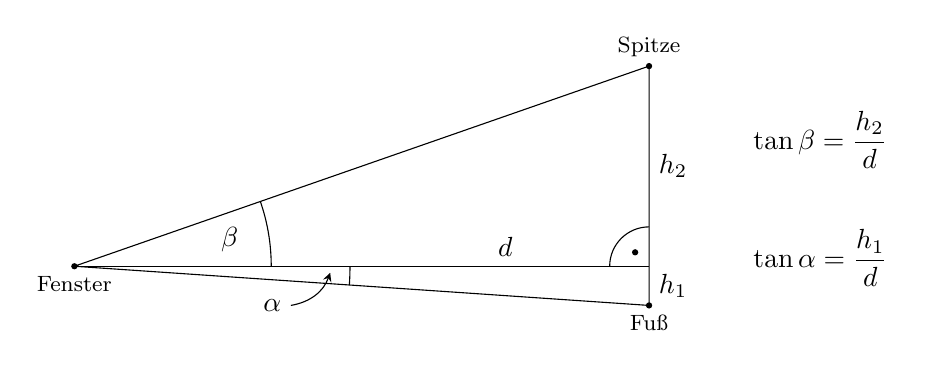
\begin{tikzpicture}[scale=0.05]
      \coordinate (A) at (  0.00,  9.95);
      \coordinate (B) at (145.95,  0.00);
      \coordinate (C) at (145.95, 60.78);
      \coordinate (D) at (145.95,  9.95);
      \fill (A) circle[radius=8mm];
      \fill (B) circle[radius=8mm];
      \fill (C) circle[radius=8mm];
      \draw (A) -- (B) -- (C) -- cycle;
      \draw (A) -- (D);
      \node[below]  at (A) {{\footnotesize Fenster}};
      \node[above] at (C) {{\footnotesize Spitze}};
      \node[below] at (B) {{\footnotesize Fuß}};
      \path (B) -- node[right] {$h_{1}$} (D);
      \path (D) -- node[right] {$h_{2}$} (C);
      \path (A) -- node[above, pos=0.75] {$d$} (D);
      % alpha
      \begin{scope}
        \clip (A) -- (D) -- (B) -- cycle;
        \draw (A) circle[radius=70cm];
      \end{scope}
      \draw[->, >=stealth] (55, 0) node[left] {$\alpha$} to[out=10, in=250] ([shift={(0, 10)}]-1.5:65);
      % beta
      \begin{scope}
        \clip (A) -- (D) -- (C) -- cycle;
        \draw (A) circle[radius=50cm];
        \node at ([shift={(0, 10)}]9.6:40) {$\beta$};
      \end{scope}
      % rechter Winkel
      \begin{scope}
        \clip (A) -- (D) -- (C) -- cycle;
        \draw (D) circle[radius=10cm];
        \fill ([shift={(135:5cm)}]D) circle[radius=8mm];
      \end{scope}
      \node[right] at (170, 42) {$\displaystyle\tan\beta=\frac{h_{2}}{d}$};
      \node[right] at (170, 12) {$\displaystyle\tan\alpha=\frac{h_{1}}{d}$};
    \end{tikzpicture}
  }
  \ifproblem\problem
    Von einem \SI{9.95}{\metre} hoch gelegenen Fenster eines
    Hauses sieht man die Spitze eines Turmes unter dem Höhenwinkel
    \SI{19.2}{\degree}, den Fuß des Turms unter dem Tiefenwinkel
    \SI{3.9}{\degree}. Wie hoch ist der Turm und wie weit ist er
    vom Haus entfernt, wenn er mit diesem auf derselben
    waagerechten Ebene steht?
  \fi
  \ifoutline\outline
    \begin{center}
      \zeichnung
    \end{center}
  \fi
  \ifoutcome\outcome
    \begin{center}
      \zeichnung
    \end{center}

    Die Entfernung $d$ lässt sich aus der Fensterhöhe $h_{1}$ und dem Tiefenwinkel $\alpha$ berechnen:
    \begin{equation*}
      d=\frac{h_{1}}{\tan\alpha}\approx\simeter{145.95}
    \end{equation*}

    Aus der Entfernung $d$ und dem Höhenwinkel $\beta$ ergibt sich die Hilfsgröße $h_{2}$:
    \begin{equation*}
      h_{2}=d\cdot\tan\beta\approx\simeter{50.83}
    \end{equation*}

    Also besitzt der Turm insgesamt eine Höhe von ca. \simeter{60.78}.
  \fi
\end{exercise}
